% Created by tikzDevice version 0.12.3 on 2020-05-24 14:46:59
% !TEX encoding = UTF-8 Unicode
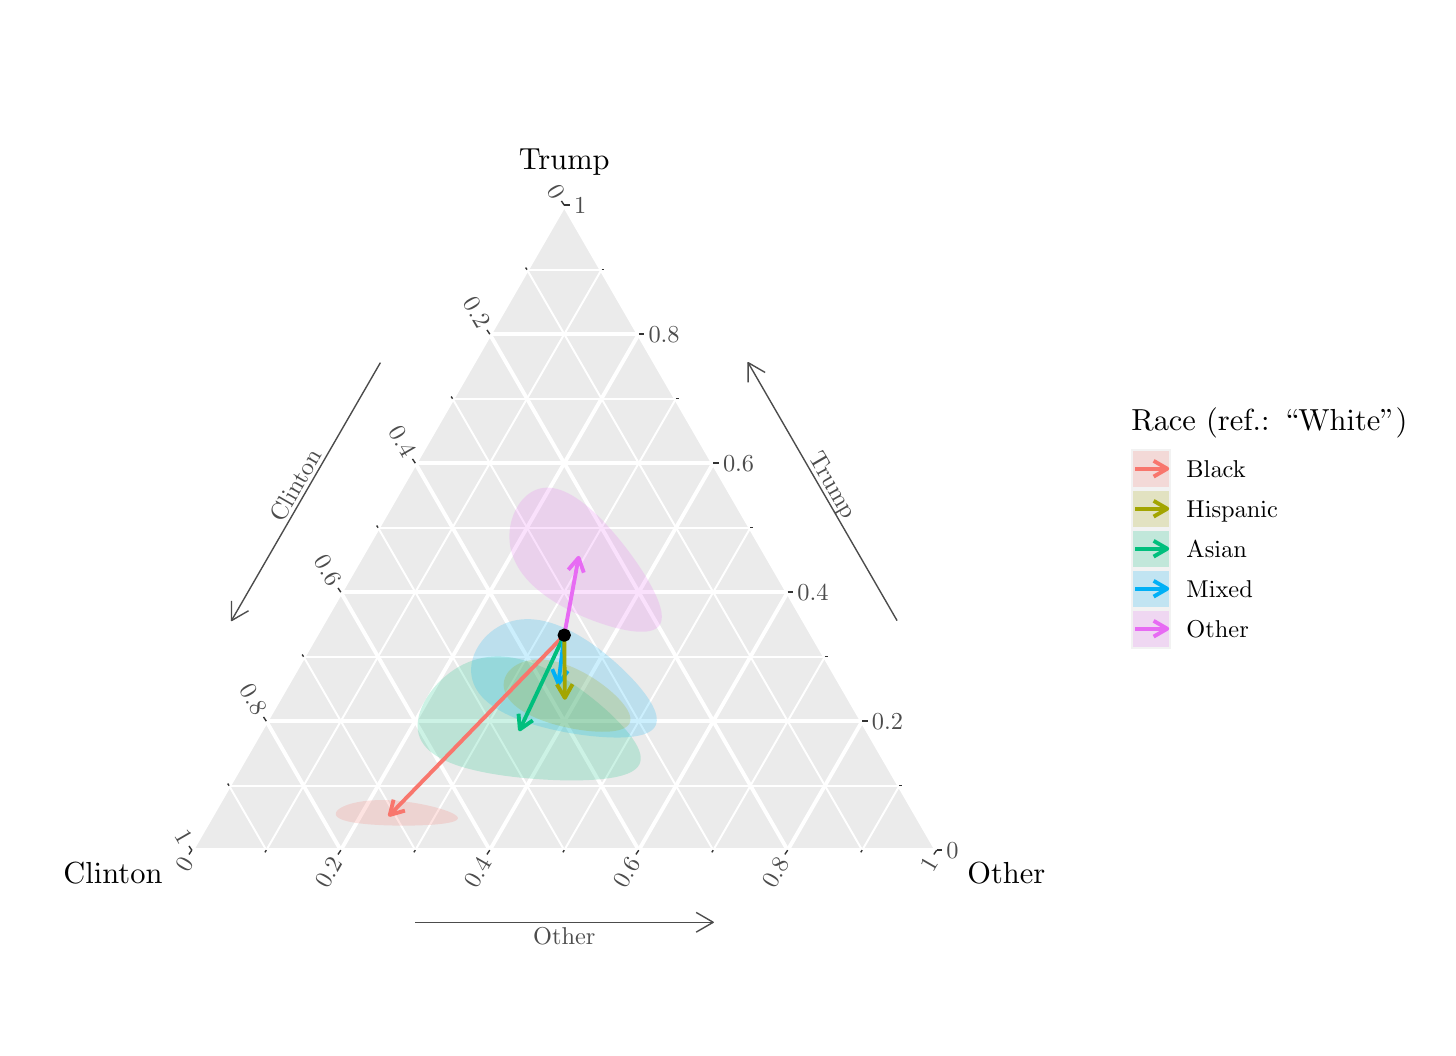
\begin{tikzpicture}[x=1pt,y=1pt]
\definecolor{fillColor}{RGB}{255,255,255}
\path[use as bounding box,fill=fillColor,fill opacity=0.00] (0,0) rectangle (505.89,361.35);
\begin{scope}
\path[clip] (  0.00, 12.02) rectangle (505.89,349.33);
\definecolor{drawColor}{RGB}{255,255,255}
\definecolor{fillColor}{RGB}{255,255,255}

\path[draw=drawColor,line width= 1.4pt,line join=round,line cap=round,fill=fillColor] (  0.00, 12.02) rectangle (505.89,349.33);
\end{scope}
\begin{scope}
\path[clip] (  5.50, 17.52) rectangle (382.29,343.83);
\definecolor{fillColor}{gray}{0.92}

\path[fill=fillColor] (193.89,297.21) --
	( 59.33, 64.14) --
	(328.46, 64.14) --
	cycle;
\definecolor{drawColor}{RGB}{255,255,255}

\path[draw=drawColor,line width= 0.7pt,line join=round] (315.00, 87.44) -- ( 72.78, 87.44);

\path[draw=drawColor,line width= 0.7pt,line join=round] (288.09,134.06) -- ( 99.70,134.06);

\path[draw=drawColor,line width= 0.7pt,line join=round] (261.18,180.68) -- (126.61,180.68);

\path[draw=drawColor,line width= 0.7pt,line join=round] (234.26,227.29) -- (153.52,227.29);

\path[draw=drawColor,line width= 0.7pt,line join=round] (207.35,273.91) -- (180.44,273.91);

\path[draw=drawColor,line width= 0.7pt,line join=round] (180.44,273.91) -- (301.55, 64.14);

\path[draw=drawColor,line width= 0.7pt,line join=round] (153.52,227.29) -- (247.72, 64.14);

\path[draw=drawColor,line width= 0.7pt,line join=round] (126.61,180.68) -- (193.89, 64.14);

\path[draw=drawColor,line width= 0.7pt,line join=round] ( 99.70,134.06) -- (140.07, 64.14);

\path[draw=drawColor,line width= 0.7pt,line join=round] ( 72.78, 87.44) -- ( 86.24, 64.14);

\path[draw=drawColor,line width= 0.7pt,line join=round] ( 86.24, 64.14) -- (207.35,273.91);

\path[draw=drawColor,line width= 0.7pt,line join=round] (140.07, 64.14) -- (234.26,227.29);

\path[draw=drawColor,line width= 0.7pt,line join=round] (193.89, 64.14) -- (261.18,180.68);

\path[draw=drawColor,line width= 0.7pt,line join=round] (247.72, 64.14) -- (288.09,134.06);

\path[draw=drawColor,line width= 0.7pt,line join=round] (301.55, 64.14) -- (315.00, 87.44);

\path[draw=drawColor,line width= 1.4pt,line join=round] (328.46, 64.14) -- ( 59.33, 64.14);

\path[draw=drawColor,line width= 1.4pt,line join=round] (301.55,110.75) -- ( 86.24,110.75);

\path[draw=drawColor,line width= 1.4pt,line join=round] (274.63,157.37) -- (113.15,157.37);

\path[draw=drawColor,line width= 1.4pt,line join=round] (247.72,203.98) -- (140.07,203.98);

\path[draw=drawColor,line width= 1.4pt,line join=round] (220.81,250.60) -- (166.98,250.60);

\path[draw=drawColor,line width= 1.4pt,line join=round] (193.89,297.21) -- (193.89,297.21);

\path[draw=drawColor,line width= 1.4pt,line join=round] (193.89,297.21) -- (328.46, 64.14);

\path[draw=drawColor,line width= 1.4pt,line join=round] (166.98,250.60) -- (274.63, 64.14);

\path[draw=drawColor,line width= 1.4pt,line join=round] (140.07,203.98) -- (220.81, 64.14);

\path[draw=drawColor,line width= 1.4pt,line join=round] (113.15,157.37) -- (166.98, 64.14);

\path[draw=drawColor,line width= 1.4pt,line join=round] ( 86.24,110.75) -- (113.15, 64.14);

\path[draw=drawColor,line width= 1.4pt,line join=round] ( 59.33, 64.14) -- ( 59.33, 64.14);

\path[draw=drawColor,line width= 1.4pt,line join=round] ( 59.33, 64.14) -- (193.89,297.21);

\path[draw=drawColor,line width= 1.4pt,line join=round] (113.15, 64.14) -- (220.81,250.60);

\path[draw=drawColor,line width= 1.4pt,line join=round] (166.98, 64.14) -- (247.72,203.98);

\path[draw=drawColor,line width= 1.4pt,line join=round] (220.81, 64.14) -- (274.63,157.37);

\path[draw=drawColor,line width= 1.4pt,line join=round] (274.63, 64.14) -- (301.55,110.75);

\path[draw=drawColor,line width= 1.4pt,line join=round] (328.46, 64.14) -- (328.46, 64.14);
\definecolor{fillColor}{RGB}{248,118,109}

\path[fill=fillColor,fill opacity=0.20] (149.10, 79.11) --
	(150.10, 78.80) --
	(151.04, 78.48) --
	(151.89, 78.17) --
	(152.67, 77.85) --
	(153.36, 77.54) --
	(153.95, 77.23) --
	(154.45, 76.93) --
	(154.85, 76.63) --
	(155.15, 76.35) --
	(155.34, 76.07) --
	(155.43, 75.80) --
	(155.41, 75.54) --
	(155.29, 75.30) --
	(155.05, 75.06) --
	(154.71, 74.84) --
	(154.27, 74.63) --
	(153.72, 74.44) --
	(153.07, 74.25) --
	(152.33, 74.08) --
	(151.49, 73.93) --
	(150.57, 73.78) --
	(149.56, 73.65) --
	(148.48, 73.53) --
	(147.32, 73.42) --
	(146.10, 73.33) --
	(144.82, 73.25) --
	(143.49, 73.18) --
	(142.12, 73.12) --
	(140.71, 73.07) --
	(139.27, 73.04) --
	(137.81, 73.02) --
	(136.34, 73.01) --
	(134.86, 73.01) --
	(133.38, 73.02) --
	(131.92, 73.05) --
	(130.46, 73.09) --
	(129.03, 73.13) --
	(127.63, 73.19) --
	(126.26, 73.27) --
	(124.93, 73.35) --
	(123.65, 73.44) --
	(122.41, 73.55) --
	(121.23, 73.67) --
	(120.10, 73.80) --
	(119.04, 73.94) --
	(118.03, 74.09) --
	(117.09, 74.26) --
	(116.22, 74.43) --
	(115.42, 74.62) --
	(114.69, 74.82) --
	(114.03, 75.03) --
	(113.44, 75.25) --
	(112.92, 75.48) --
	(112.47, 75.73) --
	(112.10, 75.98) --
	(111.80, 76.24) --
	(111.58, 76.51) --
	(111.42, 76.79) --
	(111.34, 77.07) --
	(111.33, 77.36) --
	(111.39, 77.66) --
	(111.52, 77.95) --
	(111.72, 78.26) --
	(111.99, 78.56) --
	(112.32, 78.86) --
	(112.73, 79.16) --
	(113.19, 79.46) --
	(113.73, 79.75) --
	(114.32, 80.03) --
	(114.98, 80.31) --
	(115.70, 80.57) --
	(116.48, 80.82) --
	(117.31, 81.06) --
	(118.20, 81.27) --
	(119.15, 81.47) --
	(120.14, 81.65) --
	(121.19, 81.81) --
	(122.28, 81.95) --
	(123.42, 82.06) --
	(124.60, 82.14) --
	(125.81, 82.20) --
	(127.07, 82.23) --
	(128.35, 82.24) --
	(129.66, 82.21) --
	(131.00, 82.16) --
	(132.35, 82.08) --
	(133.72, 81.98) --
	(135.09, 81.84) --
	(136.47, 81.69) --
	(137.85, 81.51) --
	(139.22, 81.30) --
	(140.57, 81.08) --
	(141.90, 80.84) --
	(143.21, 80.58) --
	(144.48, 80.31) --
	(145.71, 80.02) --
	(146.89, 79.73) --
	(148.03, 79.42) --
	(149.10, 79.11) --
	cycle;
\definecolor{fillColor}{RGB}{0,191,125}

\path[fill=fillColor,fill opacity=0.20] (210.21,113.75) --
	(211.94,112.09) --
	(213.55,110.46) --
	(215.04,108.86) --
	(216.40,107.31) --
	(217.61,105.80) --
	(218.67,104.35) --
	(219.57,102.96) --
	(220.31,101.63) --
	(220.88,100.38) --
	(221.28, 99.19) --
	(221.49, 98.07) --
	(221.53, 97.03) --
	(221.38, 96.06) --
	(221.04, 95.16) --
	(220.52, 94.33) --
	(219.81, 93.57) --
	(218.91, 92.89) --
	(217.84, 92.27) --
	(216.58, 91.71) --
	(215.14, 91.22) --
	(213.53, 90.79) --
	(211.75, 90.42) --
	(209.81, 90.11) --
	(207.72, 89.85) --
	(205.48, 89.65) --
	(203.12, 89.50) --
	(200.63, 89.40) --
	(198.03, 89.35) --
	(195.34, 89.35) --
	(192.57, 89.40) --
	(189.74, 89.50) --
	(186.87, 89.64) --
	(183.96, 89.83) --
	(181.05, 90.06) --
	(178.14, 90.33) --
	(175.26, 90.66) --
	(172.41, 91.02) --
	(169.63, 91.44) --
	(166.91, 91.89) --
	(164.28, 92.40) --
	(161.76, 92.95) --
	(159.34, 93.55) --
	(157.05, 94.19) --
	(154.89, 94.89) --
	(152.88, 95.64) --
	(151.01, 96.44) --
	(149.29, 97.28) --
	(147.73, 98.19) --
	(146.33, 99.14) --
	(145.09,100.14) --
	(144.01,101.20) --
	(143.10,102.31) --
	(142.34,103.47) --
	(141.75,104.68) --
	(141.31,105.93) --
	(141.03,107.23) --
	(140.90,108.57) --
	(140.92,109.95) --
	(141.08,111.36) --
	(141.38,112.79) --
	(141.81,114.25) --
	(142.37,115.72) --
	(143.06,117.19) --
	(143.86,118.67) --
	(144.78,120.13) --
	(145.81,121.58) --
	(146.93,122.99) --
	(148.16,124.37) --
	(149.48,125.69) --
	(150.89,126.96) --
	(152.38,128.15) --
	(153.94,129.26) --
	(155.58,130.28) --
	(157.30,131.20) --
	(159.07,132.01) --
	(160.91,132.70) --
	(162.81,133.26) --
	(164.76,133.69) --
	(166.77,133.98) --
	(168.82,134.13) --
	(170.92,134.13) --
	(173.06,133.98) --
	(175.25,133.69) --
	(177.46,133.24) --
	(179.70,132.66) --
	(181.97,131.93) --
	(184.26,131.06) --
	(186.56,130.07) --
	(188.87,128.96) --
	(191.17,127.74) --
	(193.46,126.41) --
	(195.74,125.00) --
	(197.98,123.52) --
	(200.18,121.97) --
	(202.33,120.37) --
	(204.42,118.74) --
	(206.44,117.08) --
	(208.37,115.41) --
	(210.21,113.75) --
	cycle;
\definecolor{fillColor}{RGB}{0,176,246}

\path[fill=fillColor,fill opacity=0.20] (218.20,126.39) --
	(219.61,124.86) --
	(220.93,123.35) --
	(222.13,121.87) --
	(223.23,120.44) --
	(224.21,119.04) --
	(225.06,117.70) --
	(225.79,116.42) --
	(226.38,115.19) --
	(226.83,114.03) --
	(227.14,112.93) --
	(227.30,111.90) --
	(227.32,110.94) --
	(227.19,110.05) --
	(226.91,109.24) --
	(226.48,108.49) --
	(225.89,107.82) --
	(225.16,107.22) --
	(224.28,106.69) --
	(223.25,106.23) --
	(222.07,105.83) --
	(220.76,105.51) --
	(219.31,105.25) --
	(217.73,105.06) --
	(216.02,104.92) --
	(214.20,104.85) --
	(212.27,104.84) --
	(210.24,104.89) --
	(208.13,105.00) --
	(205.93,105.16) --
	(203.67,105.38) --
	(201.36,105.65) --
	(199.00,105.97) --
	(196.62,106.35) --
	(194.22,106.77) --
	(191.83,107.24) --
	(189.45,107.77) --
	(187.09,108.34) --
	(184.78,108.95) --
	(182.52,109.61) --
	(180.32,110.32) --
	(178.21,111.07) --
	(176.18,111.87) --
	(174.25,112.71) --
	(172.42,113.59) --
	(170.71,114.52) --
	(169.11,115.48) --
	(167.64,116.49) --
	(166.30,117.54) --
	(165.09,118.62) --
	(164.01,119.74) --
	(163.07,120.89) --
	(162.27,122.08) --
	(161.60,123.29) --
	(161.07,124.53) --
	(160.67,125.80) --
	(160.40,127.08) --
	(160.25,128.37) --
	(160.24,129.68) --
	(160.34,130.98) --
	(160.56,132.29) --
	(160.90,133.59) --
	(161.35,134.87) --
	(161.90,136.13) --
	(162.55,137.37) --
	(163.31,138.56) --
	(164.15,139.72) --
	(165.08,140.83) --
	(166.10,141.87) --
	(167.20,142.85) --
	(168.37,143.76) --
	(169.62,144.59) --
	(170.93,145.33) --
	(172.31,145.98) --
	(173.76,146.53) --
	(175.26,146.97) --
	(176.82,147.30) --
	(178.43,147.52) --
	(180.09,147.62) --
	(181.80,147.59) --
	(183.55,147.45) --
	(185.34,147.19) --
	(187.16,146.80) --
	(189.02,146.29) --
	(190.90,145.66) --
	(192.81,144.92) --
	(194.73,144.06) --
	(196.67,143.10) --
	(198.61,142.04) --
	(200.55,140.89) --
	(202.48,139.66) --
	(204.39,138.35) --
	(206.29,136.98) --
	(208.15,135.55) --
	(209.97,134.07) --
	(211.75,132.56) --
	(213.47,131.03) --
	(215.12,129.48) --
	(216.70,127.93) --
	(218.20,126.39) --
	cycle;
\definecolor{fillColor}{RGB}{163,165,0}

\path[fill=fillColor,fill opacity=0.20] (212.12,120.32) --
	(213.04,119.43) --
	(213.89,118.54) --
	(214.66,117.67) --
	(215.36,116.81) --
	(215.98,115.97) --
	(216.51,115.16) --
	(216.95,114.38) --
	(217.31,113.63) --
	(217.57,112.91) --
	(217.73,112.23) --
	(217.80,111.58) --
	(217.77,110.97) --
	(217.64,110.41) --
	(217.42,109.88) --
	(217.09,109.40) --
	(216.67,108.96) --
	(216.15,108.56) --
	(215.53,108.20) --
	(214.83,107.89) --
	(214.03,107.63) --
	(213.14,107.40) --
	(212.17,107.23) --
	(211.12,107.09) --
	(209.99,106.99) --
	(208.79,106.94) --
	(207.53,106.93) --
	(206.20,106.96) --
	(204.82,107.03) --
	(203.40,107.14) --
	(201.93,107.29) --
	(200.43,107.48) --
	(198.91,107.71) --
	(197.36,107.97) --
	(195.81,108.26) --
	(194.25,108.59) --
	(192.70,108.96) --
	(191.16,109.36) --
	(189.64,109.79) --
	(188.15,110.25) --
	(186.69,110.75) --
	(185.28,111.27) --
	(183.91,111.82) --
	(182.60,112.40) --
	(181.35,113.00) --
	(180.16,113.63) --
	(179.04,114.29) --
	(177.99,114.96) --
	(177.02,115.66) --
	(176.13,116.38) --
	(175.33,117.11) --
	(174.61,117.86) --
	(173.97,118.62) --
	(173.42,119.40) --
	(172.97,120.18) --
	(172.60,120.97) --
	(172.32,121.76) --
	(172.13,122.55) --
	(172.02,123.34) --
	(172.01,124.12) --
	(172.08,124.90) --
	(172.23,125.66) --
	(172.46,126.40) --
	(172.78,127.12) --
	(173.17,127.82) --
	(173.64,128.49) --
	(174.19,129.13) --
	(174.80,129.74) --
	(175.48,130.30) --
	(176.23,130.82) --
	(177.04,131.29) --
	(177.92,131.71) --
	(178.85,132.08) --
	(179.83,132.39) --
	(180.86,132.64) --
	(181.95,132.84) --
	(183.08,132.96) --
	(184.25,133.02) --
	(185.45,133.02) --
	(186.69,132.95) --
	(187.97,132.81) --
	(189.27,132.61) --
	(190.59,132.33) --
	(191.93,132.00) --
	(193.29,131.60) --
	(194.66,131.13) --
	(196.03,130.61) --
	(197.40,130.04) --
	(198.78,129.41) --
	(200.14,128.73) --
	(201.48,128.01) --
	(202.81,127.25) --
	(204.12,126.46) --
	(205.39,125.63) --
	(206.63,124.78) --
	(207.83,123.91) --
	(208.98,123.02) --
	(210.08,122.12) --
	(211.13,121.22) --
	(212.12,120.32) --
	cycle;
\definecolor{fillColor}{RGB}{231,107,243}

\path[fill=fillColor,fill opacity=0.20] (220.68,167.20) --
	(221.91,165.33) --
	(223.08,163.49) --
	(224.16,161.68) --
	(225.15,159.92) --
	(226.05,158.23) --
	(226.84,156.59) --
	(227.53,155.03) --
	(228.10,153.55) --
	(228.55,152.16) --
	(228.88,150.86) --
	(229.08,149.65) --
	(229.15,148.54) --
	(229.08,147.53) --
	(228.88,146.62) --
	(228.55,145.81) --
	(228.08,145.11) --
	(227.47,144.52) --
	(226.72,144.03) --
	(225.85,143.64) --
	(224.84,143.35) --
	(223.70,143.16) --
	(222.45,143.07) --
	(221.07,143.07) --
	(219.59,143.17) --
	(218.00,143.35) --
	(216.32,143.63) --
	(214.55,143.98) --
	(212.71,144.42) --
	(210.81,144.93) --
	(208.85,145.52) --
	(206.85,146.18) --
	(204.82,146.90) --
	(202.77,147.69) --
	(200.73,148.53) --
	(198.69,149.44) --
	(196.68,150.39) --
	(194.70,151.40) --
	(192.77,152.45) --
	(190.89,153.55) --
	(189.09,154.70) --
	(187.36,155.88) --
	(185.72,157.10) --
	(184.17,158.35) --
	(182.73,159.64) --
	(181.38,160.96) --
	(180.15,162.30) --
	(179.03,163.67) --
	(178.03,165.06) --
	(177.14,166.48) --
	(176.37,167.91) --
	(175.71,169.35) --
	(175.17,170.80) --
	(174.73,172.26) --
	(174.41,173.72) --
	(174.20,175.17) --
	(174.09,176.62) --
	(174.07,178.06) --
	(174.16,179.48) --
	(174.33,180.87) --
	(174.59,182.24) --
	(174.93,183.57) --
	(175.36,184.86) --
	(175.85,186.10) --
	(176.42,187.29) --
	(177.06,188.41) --
	(177.75,189.47) --
	(178.51,190.46) --
	(179.32,191.37) --
	(180.19,192.19) --
	(181.11,192.92) --
	(182.07,193.56) --
	(183.09,194.09) --
	(184.14,194.52) --
	(185.24,194.84) --
	(186.39,195.04) --
	(187.57,195.13) --
	(188.79,195.09) --
	(190.05,194.93) --
	(191.34,194.64) --
	(192.68,194.23) --
	(194.04,193.69) --
	(195.44,193.03) --
	(196.87,192.24) --
	(198.32,191.32) --
	(199.81,190.29) --
	(201.31,189.14) --
	(202.83,187.89) --
	(204.37,186.52) --
	(205.92,185.07) --
	(207.48,183.52) --
	(209.04,181.89) --
	(210.59,180.19) --
	(212.13,178.43) --
	(213.64,176.62) --
	(215.14,174.77) --
	(216.59,172.89) --
	(218.01,170.99) --
	(219.37,169.09) --
	(220.68,167.20) --
	cycle;
\definecolor{drawColor}{RGB}{248,118,109}

\path[draw=drawColor,line width= 1.4pt,line join=round] (193.89,141.83) -- (130.84, 76.87);

\path[draw=drawColor,line width= 1.4pt,line join=round] (132.23, 82.39) --
	(130.84, 76.87) --
	(136.31, 78.42);
\definecolor{drawColor}{RGB}{0,191,125}

\path[draw=drawColor,line width= 1.4pt,line join=round] (193.89,141.83) -- (177.85,107.78);

\path[draw=drawColor,line width= 1.4pt,line join=round] (177.37,113.45) --
	(177.85,107.78) --
	(182.52,111.03);
\definecolor{drawColor}{RGB}{0,176,246}

\path[draw=drawColor,line width= 1.4pt,line join=round] (193.89,141.83) -- (191.79,124.33);

\path[draw=drawColor,line width= 1.4pt,line join=round] (189.55,129.57) --
	(191.79,124.33) --
	(195.20,128.89);
\definecolor{drawColor}{RGB}{163,165,0}

\path[draw=drawColor,line width= 1.4pt,line join=round] (193.89,141.83) -- (194.11,119.17);

\path[draw=drawColor,line width= 1.4pt,line join=round] (191.21,124.07) --
	(194.11,119.17) --
	(196.90,124.13);
\definecolor{drawColor}{RGB}{231,107,243}

\path[draw=drawColor,line width= 1.4pt,line join=round] (193.89,141.83) -- (199.06,169.79);

\path[draw=drawColor,line width= 1.4pt,line join=round] (200.96,164.43) --
	(199.06,169.79) --
	(195.36,165.46);
\definecolor{drawColor}{RGB}{0,0,0}
\definecolor{fillColor}{RGB}{0,0,0}

\path[draw=drawColor,line width= 0.9pt,line join=round,line cap=round,fill=fillColor] (193.89,141.83) circle (  1.96);
\definecolor{fillColor}{RGB}{255,255,255}

\path[fill=fillColor] (  5.50, 17.52) --
	(  5.50,343.83) --
	(193.89,343.83) --
	(193.89,297.21) --
	( 59.33, 64.14) --
	(328.46, 64.14) --
	(193.89,297.21) --
	(193.89,343.83) --
	(382.29,343.83) --
	(382.29, 17.52) --
	(  5.50, 17.52) --
	cycle;
\end{scope}
\begin{scope}
\path[clip] (  5.50, 17.52) rectangle (382.29,343.83);

\path[] (  5.50, 17.52) --
	(  5.50,343.83) --
	(382.29,343.83) --
	(382.29, 17.52) --
	(  5.50, 17.52) --
	(  5.50, 17.52);
\end{scope}
\begin{scope}
\path[clip] (  5.50, 17.52) rectangle (382.29,343.83);
\definecolor{drawColor}{gray}{0.20}

\path[draw=drawColor,line width= 0.5pt,line join=round] (328.46, 64.14) -- (330.51, 64.14);

\path[draw=drawColor,line width= 0.5pt,line join=round] (301.55,110.75) -- (303.59,110.75);

\path[draw=drawColor,line width= 0.5pt,line join=round] (274.63,157.37) -- (276.68,157.37);

\path[draw=drawColor,line width= 0.5pt,line join=round] (247.72,203.98) -- (249.77,203.98);

\path[draw=drawColor,line width= 0.5pt,line join=round] (220.81,250.60) -- (222.85,250.60);

\path[draw=drawColor,line width= 0.5pt,line join=round] (193.89,297.21) -- (195.94,297.21);

\path[draw=drawColor,line width= 0.5pt,line join=round] (315.00, 87.44) -- (316.03, 87.44);

\path[draw=drawColor,line width= 0.5pt,line join=round] (288.09,134.06) -- (289.11,134.06);

\path[draw=drawColor,line width= 0.5pt,line join=round] (261.18,180.68) -- (262.20,180.68);

\path[draw=drawColor,line width= 0.5pt,line join=round] (234.26,227.29) -- (235.29,227.29);

\path[draw=drawColor,line width= 0.5pt,line join=round] (207.35,273.91) -- (208.37,273.91);

\path[draw=drawColor,line width= 0.5pt,line join=round] (193.89,297.21) -- (192.87,298.75);

\path[draw=drawColor,line width= 0.5pt,line join=round] (166.98,250.60) -- (165.96,252.13);

\path[draw=drawColor,line width= 0.5pt,line join=round] (140.07,203.98) -- (139.04,205.52);

\path[draw=drawColor,line width= 0.5pt,line join=round] (113.15,157.37) -- (112.13,158.90);

\path[draw=drawColor,line width= 0.5pt,line join=round] ( 86.24,110.75) -- ( 85.22,112.29);

\path[draw=drawColor,line width= 0.5pt,line join=round] ( 59.33, 64.14) -- ( 58.30, 65.67);

\path[draw=drawColor,line width= 0.5pt,line join=round] (180.44,273.91) -- (179.92,274.67);

\path[draw=drawColor,line width= 0.5pt,line join=round] (153.52,227.29) -- (153.01,228.06);

\path[draw=drawColor,line width= 0.5pt,line join=round] (126.61,180.68) -- (126.10,181.44);

\path[draw=drawColor,line width= 0.5pt,line join=round] ( 99.70,134.06) -- ( 99.18,134.83);

\path[draw=drawColor,line width= 0.5pt,line join=round] ( 72.78, 87.44) -- ( 72.27, 88.21);

\path[draw=drawColor,line width= 0.5pt,line join=round] ( 59.33, 64.14) -- ( 58.30, 62.60);

\path[draw=drawColor,line width= 0.5pt,line join=round] (113.15, 64.14) -- (112.13, 62.60);

\path[draw=drawColor,line width= 0.5pt,line join=round] (166.98, 64.14) -- (165.96, 62.60);

\path[draw=drawColor,line width= 0.5pt,line join=round] (220.81, 64.14) -- (219.78, 62.60);

\path[draw=drawColor,line width= 0.5pt,line join=round] (274.63, 64.14) -- (273.61, 62.60);

\path[draw=drawColor,line width= 0.5pt,line join=round] (328.46, 64.14) -- (327.43, 62.60);

\path[draw=drawColor,line width= 0.5pt,line join=round] ( 86.24, 64.14) -- ( 85.73, 63.37);

\path[draw=drawColor,line width= 0.5pt,line join=round] (140.07, 64.14) -- (139.55, 63.37);

\path[draw=drawColor,line width= 0.5pt,line join=round] (193.89, 64.14) -- (193.38, 63.37);

\path[draw=drawColor,line width= 0.5pt,line join=round] (247.72, 64.14) -- (247.21, 63.37);

\path[draw=drawColor,line width= 0.5pt,line join=round] (301.55, 64.14) -- (301.03, 63.37);
\definecolor{drawColor}{gray}{0.30}

\node[text=drawColor,anchor=base west,inner sep=0pt, outer sep=0pt, scale=  0.88] at (332.00, 61.11) {0};

\node[text=drawColor,anchor=base west,inner sep=0pt, outer sep=0pt, scale=  0.88] at (305.08,107.72) {0.2};

\node[text=drawColor,anchor=base west,inner sep=0pt, outer sep=0pt, scale=  0.88] at (278.17,154.34) {0.4};

\node[text=drawColor,anchor=base west,inner sep=0pt, outer sep=0pt, scale=  0.88] at (251.26,200.95) {0.6};

\node[text=drawColor,anchor=base west,inner sep=0pt, outer sep=0pt, scale=  0.88] at (224.34,247.57) {0.8};

\node[text=drawColor,anchor=base west,inner sep=0pt, outer sep=0pt, scale=  0.88] at (197.43,294.18) {1};

\node[text=drawColor,rotate=-60.00,anchor=base east,inner sep=0pt, outer sep=0pt, scale=  0.88] at (189.50,298.80) {0};

\node[text=drawColor,rotate=-60.00,anchor=base east,inner sep=0pt, outer sep=0pt, scale=  0.88] at (162.59,252.18) {0.2};

\node[text=drawColor,rotate=-60.00,anchor=base east,inner sep=0pt, outer sep=0pt, scale=  0.88] at (135.67,205.57) {0.4};

\node[text=drawColor,rotate=-60.00,anchor=base east,inner sep=0pt, outer sep=0pt, scale=  0.88] at (108.76,158.95) {0.6};

\node[text=drawColor,rotate=-60.00,anchor=base east,inner sep=0pt, outer sep=0pt, scale=  0.88] at ( 81.85,112.34) {0.8};

\node[text=drawColor,rotate=-60.00,anchor=base east,inner sep=0pt, outer sep=0pt, scale=  0.88] at ( 54.93, 65.72) {1};

\node[text=drawColor,rotate= 60.00,anchor=base east,inner sep=0pt, outer sep=0pt, scale=  0.88] at ( 60.18, 59.52) {0};

\node[text=drawColor,rotate= 60.00,anchor=base east,inner sep=0pt, outer sep=0pt, scale=  0.88] at (114.01, 59.52) {0.2};

\node[text=drawColor,rotate= 60.00,anchor=base east,inner sep=0pt, outer sep=0pt, scale=  0.88] at (167.83, 59.52) {0.4};

\node[text=drawColor,rotate= 60.00,anchor=base east,inner sep=0pt, outer sep=0pt, scale=  0.88] at (221.66, 59.52) {0.6};

\node[text=drawColor,rotate= 60.00,anchor=base east,inner sep=0pt, outer sep=0pt, scale=  0.88] at (275.49, 59.52) {0.8};

\node[text=drawColor,rotate= 60.00,anchor=base east,inner sep=0pt, outer sep=0pt, scale=  0.88] at (329.31, 59.52) {1};

\path[draw=drawColor,line width= 0.5pt,line join=round] (314.15,147.09) -- (260.32,240.32);

\path[draw=drawColor,line width= 0.5pt,line join=round] (266.48,236.76) --
	(260.32,240.32) --
	(260.32,233.21);

\path[draw=drawColor,line width= 0.5pt,line join=round] (127.46,240.32) -- ( 73.64,147.09);

\path[draw=drawColor,line width= 0.5pt,line join=round] ( 73.64,154.20) --
	( 73.64,147.09) --
	( 79.80,150.65);

\path[draw=drawColor,line width= 0.5pt,line join=round] (140.07, 38.08) -- (247.72, 38.08);

\path[draw=drawColor,line width= 0.5pt,line join=round] (241.56, 34.52) --
	(247.72, 38.08) --
	(241.56, 41.64);

\node[text=drawColor,rotate=-60.00,anchor=base,inner sep=0pt, outer sep=0pt, scale=  0.88] at (288.52,194.61) {Trump};

\node[text=drawColor,rotate= 60.00,anchor=base,inner sep=0pt, outer sep=0pt, scale=  0.88] at ( 99.26,194.61) {Clinton};

\node[text=drawColor,anchor=base,inner sep=0pt, outer sep=0pt, scale=  0.88] at (193.89, 30.21) {Other};
\definecolor{drawColor}{RGB}{0,0,0}

\node[text=drawColor,anchor=base,inner sep=0pt, outer sep=0pt, scale=  1.10] at (193.89,310.24) {Trump};

\node[text=drawColor,anchor=base east,inner sep=0pt, outer sep=0pt, scale=  1.10] at ( 48.69, 51.94) {Clinton};

\node[text=drawColor,anchor=base west,inner sep=0pt, outer sep=0pt, scale=  1.10] at (339.60, 51.94) {Other};
\end{scope}
\begin{scope}
\path[clip] (  0.00,  0.00) rectangle (505.89,361.35);
\definecolor{fillColor}{RGB}{255,255,255}

\path[fill=fillColor] (393.29,131.43) rectangle (500.39,229.92);
\end{scope}
\begin{scope}
\path[clip] (  0.00,  0.00) rectangle (505.89,361.35);
\definecolor{drawColor}{RGB}{0,0,0}

\node[text=drawColor,anchor=base west,inner sep=0pt, outer sep=0pt, scale=  1.10] at (398.79,215.77) {Race (ref.: “White”)};
\end{scope}
\begin{scope}
\path[clip] (  0.00,  0.00) rectangle (505.89,361.35);
\definecolor{fillColor}{gray}{0.95}

\path[fill=fillColor] (398.79,194.75) rectangle (413.24,209.20);
\end{scope}
\begin{scope}
\path[clip] (  0.00,  0.00) rectangle (505.89,361.35);
\definecolor{fillColor}{RGB}{248,118,109}

\path[fill=fillColor,fill opacity=0.20] (399.50,195.46) rectangle (412.53,208.49);
\end{scope}
\begin{scope}
\path[clip] (  0.00,  0.00) rectangle (505.89,361.35);
\definecolor{drawColor}{RGB}{248,118,109}

\path[draw=drawColor,line width= 1.4pt,line join=round] (400.23,201.98) -- (411.79,201.98);

\path[draw=drawColor,line width= 1.4pt,line join=round] (406.87,199.13) --
	(411.79,201.98) --
	(406.87,204.82);
\end{scope}
\begin{scope}
\path[clip] (  0.00,  0.00) rectangle (505.89,361.35);
\definecolor{fillColor}{gray}{0.95}

\path[fill=fillColor] (398.79,180.29) rectangle (413.24,194.75);
\end{scope}
\begin{scope}
\path[clip] (  0.00,  0.00) rectangle (505.89,361.35);
\definecolor{fillColor}{RGB}{163,165,0}

\path[fill=fillColor,fill opacity=0.20] (399.50,181.01) rectangle (412.53,194.04);
\end{scope}
\begin{scope}
\path[clip] (  0.00,  0.00) rectangle (505.89,361.35);
\definecolor{drawColor}{RGB}{163,165,0}

\path[draw=drawColor,line width= 1.4pt,line join=round] (400.23,187.52) -- (411.79,187.52);

\path[draw=drawColor,line width= 1.4pt,line join=round] (406.87,184.68) --
	(411.79,187.52) --
	(406.87,190.37);
\end{scope}
\begin{scope}
\path[clip] (  0.00,  0.00) rectangle (505.89,361.35);
\definecolor{fillColor}{gray}{0.95}

\path[fill=fillColor] (398.79,165.84) rectangle (413.24,180.29);
\end{scope}
\begin{scope}
\path[clip] (  0.00,  0.00) rectangle (505.89,361.35);
\definecolor{fillColor}{RGB}{0,191,125}

\path[fill=fillColor,fill opacity=0.20] (399.50,166.55) rectangle (412.53,179.58);
\end{scope}
\begin{scope}
\path[clip] (  0.00,  0.00) rectangle (505.89,361.35);
\definecolor{drawColor}{RGB}{0,191,125}

\path[draw=drawColor,line width= 1.4pt,line join=round] (400.23,173.07) -- (411.79,173.07);

\path[draw=drawColor,line width= 1.4pt,line join=round] (406.87,170.22) --
	(411.79,173.07) --
	(406.87,175.91);
\end{scope}
\begin{scope}
\path[clip] (  0.00,  0.00) rectangle (505.89,361.35);
\definecolor{fillColor}{gray}{0.95}

\path[fill=fillColor] (398.79,151.39) rectangle (413.24,165.84);
\end{scope}
\begin{scope}
\path[clip] (  0.00,  0.00) rectangle (505.89,361.35);
\definecolor{fillColor}{RGB}{0,176,246}

\path[fill=fillColor,fill opacity=0.20] (399.50,152.10) rectangle (412.53,165.13);
\end{scope}
\begin{scope}
\path[clip] (  0.00,  0.00) rectangle (505.89,361.35);
\definecolor{drawColor}{RGB}{0,176,246}

\path[draw=drawColor,line width= 1.4pt,line join=round] (400.23,158.61) -- (411.79,158.61);

\path[draw=drawColor,line width= 1.4pt,line join=round] (406.87,155.77) --
	(411.79,158.61) --
	(406.87,161.46);
\end{scope}
\begin{scope}
\path[clip] (  0.00,  0.00) rectangle (505.89,361.35);
\definecolor{fillColor}{gray}{0.95}

\path[fill=fillColor] (398.79,136.93) rectangle (413.24,151.39);
\end{scope}
\begin{scope}
\path[clip] (  0.00,  0.00) rectangle (505.89,361.35);
\definecolor{fillColor}{RGB}{231,107,243}

\path[fill=fillColor,fill opacity=0.20] (399.50,137.64) rectangle (412.53,150.68);
\end{scope}
\begin{scope}
\path[clip] (  0.00,  0.00) rectangle (505.89,361.35);
\definecolor{drawColor}{RGB}{231,107,243}

\path[draw=drawColor,line width= 1.4pt,line join=round] (400.23,144.16) -- (411.79,144.16);

\path[draw=drawColor,line width= 1.4pt,line join=round] (406.87,141.31) --
	(411.79,144.16) --
	(406.87,147.01);
\end{scope}
\begin{scope}
\path[clip] (  0.00,  0.00) rectangle (505.89,361.35);
\definecolor{drawColor}{RGB}{0,0,0}

\node[text=drawColor,anchor=base west,inner sep=0pt, outer sep=0pt, scale=  0.88] at (418.74,198.95) {Black};
\end{scope}
\begin{scope}
\path[clip] (  0.00,  0.00) rectangle (505.89,361.35);
\definecolor{drawColor}{RGB}{0,0,0}

\node[text=drawColor,anchor=base west,inner sep=0pt, outer sep=0pt, scale=  0.88] at (418.74,184.49) {Hispanic};
\end{scope}
\begin{scope}
\path[clip] (  0.00,  0.00) rectangle (505.89,361.35);
\definecolor{drawColor}{RGB}{0,0,0}

\node[text=drawColor,anchor=base west,inner sep=0pt, outer sep=0pt, scale=  0.88] at (418.74,170.04) {Asian};
\end{scope}
\begin{scope}
\path[clip] (  0.00,  0.00) rectangle (505.89,361.35);
\definecolor{drawColor}{RGB}{0,0,0}

\node[text=drawColor,anchor=base west,inner sep=0pt, outer sep=0pt, scale=  0.88] at (418.74,155.58) {Mixed};
\end{scope}
\begin{scope}
\path[clip] (  0.00,  0.00) rectangle (505.89,361.35);
\definecolor{drawColor}{RGB}{0,0,0}

\node[text=drawColor,anchor=base west,inner sep=0pt, outer sep=0pt, scale=  0.88] at (418.74,141.13) {Other};
\end{scope}
\end{tikzpicture}
